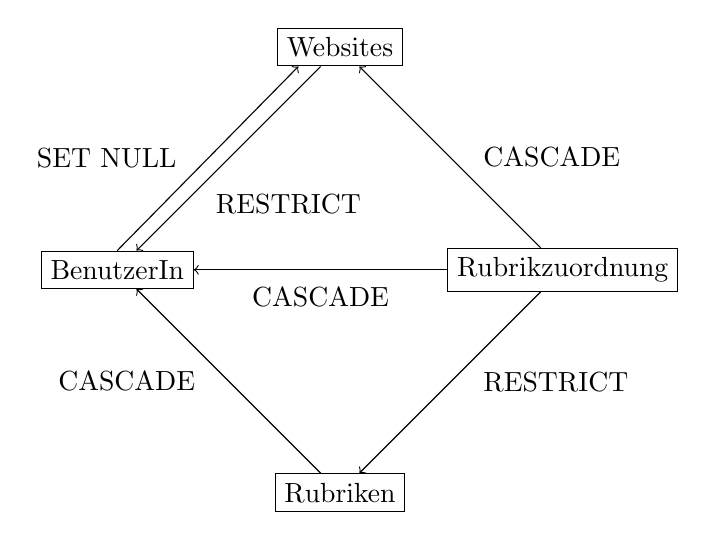
\begin{tikzpicture}[->, node distance=4cm]
\node[draw] (Websites) at (0,0) {Websites};
\node[draw] (BenutzerIn) [below left of= Websites] {BenutzerIn};
\node[draw] (Rubrikzuordnung) [below right of= Websites] {Rubrikzuordnung};
\node[draw] (Rubriken) [below right of= BenutzerIn] {Rubriken};

\draw[->] (Websites) 		-- (BenutzerIn) node [near end, right=0.30cm, fill=white] {RESTRICT};
\draw[->] (Rubrikzuordnung) -- (BenutzerIn) node [midway, below=0.1cm, fill=white] {CASCADE};
\draw[->] (Rubriken) 		-- (BenutzerIn) node [midway, left=0.30cm, fill=white] {CASCADE};;
\draw[->] (BenutzerIn.north)-- (Websites.205) node [midway, left=0.275cm, fill=white] {SET NULL};
\draw[->] (Rubrikzuordnung) -- (Websites) node [midway, right=0.30cm, fill=white] {CASCADE};;
\draw[->] (Rubrikzuordnung) -- (Rubriken) node [midway, right=0.30cm, fill=white] {RESTRICT};


\end{tikzpicture}